\documentclass{article}
\usepackage[utf8]{inputenc}
\usepackage[T1]{fontenc}
\usepackage{graphicx}
\usepackage{booktabs}
\usepackage{hyperref}
\usepackage{amsmath}

\title{Report: Cortisol vs. Cortisone Comparison}
\author{Assembler}
\date{\today}

\begin{document}

\maketitle

\section{Chemical Comparison}
\begin{center}
\begin{tabular}{|l|l|l|}
\hline
Property & Cortisol & Cortisone \\
\hline
PubChem CID & 5754 & 222786 \\
\hline
Molecular Formula & C21H30O5 & C21H28O5 \\
\hline
Molecular Weight & 362.5 & 360.4 \\
\hline
\end{tabular}
\end{center}

\section{Molecular Structures}

\subsection{Cortisol}
\begin{figure}[h]
    \centering
    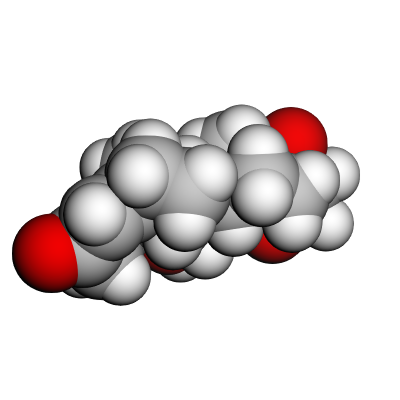
\includegraphics[width=0.4\textwidth]{output/images/cortisol_spacefilling.png}
    \caption{Cortisol Spacefilling Model}
\end{figure}

\begin{figure}[h]
    \centering
    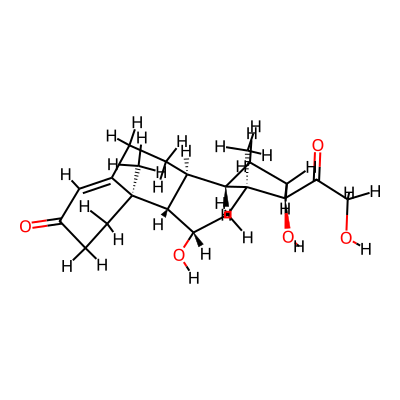
\includegraphics[width=0.4\textwidth]{output/images/cortisol_3d.png}
    \caption{Cortisol Pseudo-3D Stick Model}
\end{figure}

\subsection{Cortisone}
\begin{figure}[h]
    \centering
    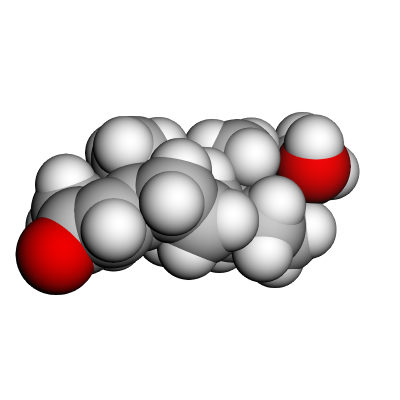
\includegraphics[width=0.4\textwidth]{output/images/cortisone_spacefilling.png}
    \caption{Cortisone Spacefilling Model}
\end{figure}

\begin{figure}[h]
    \centering
    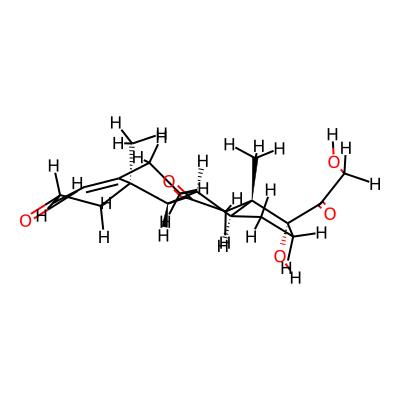
\includegraphics[width=0.4\textwidth]{output/images/cortisone_3d.png}
    \caption{Cortisone Pseudo-3D Stick Model}
\end{figure}

\# Medical Comparison: Cortisol vs. Cortisone

\#\# Overview
Cortisol and Cortisone are closely related corticosteroids, but they differ in biological activity and potency.

\#\# Biological Activity
- \textbf{Cortisol (Hydrocortisone)}: The biologically active form of the hormone. It can directly bind to glucocorticoid receptors to exert its effects.
- \textbf{Cortisone}: A prodrug (biologically inactive). It must be converted into Cortisol to become active.

\#\# Activation Pathway
The conversion of Cortisone to Cortisol is mediated by the enzyme \textbf{11$\beta$-hydroxysteroid dehydrogenase type 1 (11$\beta$-HSD1)}, which is primarily located in the liver but also found in other tissues like adipose tissue and the brain.

\#\# Relative Potency
- \textbf{Cortisol}: Relative Potency = 1 (Reference standard).
- \textbf{Cortisone}: Relative Potency ≈ 0.8. Cortisone is generally considered slightly less potent than Cortisol.

\#\# Therapeutic Use Cases
\#\#\# Cortisol (Hydrocortisone)
- \textbf{Adrenal Insufficiency}: Primary treatment for Addison's disease.
- \textbf{Acute Allergic Reactions}: Used for rapid effect in severe allergies.
- \textbf{Topical Applications}: Common in creams for skin inflammation and itching.

\#\#\# Cortisone
- \textbf{Joint and Tendon Inflammation}: Often administered via local injection (e.g., for bursitis or arthritis).
- \textbf{Systemic Inflammation}: Used orally for various autoimmune and inflammatory conditions where a prodrug approach is acceptable.

\#\# Key Differences
\begin{center}
\begin{tabular}{|l|l|l|}
\hline
Feature & Cortisol (Hydrocortisone) & Cortisone \\
\hline
**Form** & Active Hormone & Inactive Prodrug \\
\hline
**Primary Site of Action** & Systemic / Tissues & Must be activated in Liver/Tissues \\
\hline
**Half-life** & \textasciitilde{}1.5 - 2 hours & Slightly longer (due to conversion) \\
\hline
**Mineralocorticoid Activity** & High (comparatively) & Low \\
\hline
\end{tabular}
\end{center}


\# Related Organs and Proteins: Cortisol and Cortisone

\#\# Related Organs

\#\#\# Adrenal Glands
The \textbf{Adrenal Cortex}, specifically the \textit{zona fasciculata}, is the primary site of Cortisol production. In response to stress or low blood-glucose, it releases Cortisol into the bloodstream.

\#\#\# Liver
The liver is a major hub for the metabolism of these steroids. It is the primary site where \textbf{Cortisone is converted into active Cortisol} via the enzyme 11$\beta$-HSD1. It also handles the inactivation and conjugation of these hormones for excretion.

\#\#\# Hypothalamus and Pituitary Gland
These brain structures regulate Cortisol levels through the \textbf{HPA axis} (Hypothalamic-Pituitary-Adrenal axis).
- The \textbf{Hypothalamus} releases Corticotropin-releasing hormone (CRH).
- CRH stimulates the \textbf{Anterior Pituitary} to release Adrenocorticotropic hormone (ACTH).
- ACTH then signals the Adrenal Glands to produce Cortisol.

\#\#\# Kidneys
The kidneys play a crucial role in protecting the body from excess mineralocorticoid activity. While Cortisol can bind to both Glucocorticoid and Mineralocorticoid receptors, the kidneys use the enzyme \textbf{11$\beta$-HSD2} to convert Cortisol into inactive Cortisone, preventing it from over-activating Mineralocorticoid receptors in the renal tubules.

\hrulefill

\#\# Related Proteins and Enzymes

\#\#\# Enzymes: 11$\beta$-HSD System
- \textbf{11$\beta$-hydroxysteroid dehydrogenase type 1 (11$\beta$-HSD1)}: Primarily converts inactive Cortisone into active Cortisol. It is found in the liver, adipose tissue, and the brain.
- \textbf{11$\beta$-hydroxysteroid dehydrogenase type 2 (11$\beta$-HSD2)}: Primarily converts active Cortisol into inactive Cortisone. It is highly expressed in the kidneys to prevent Cortisol from over-stimulating mineralocorticoid receptors.

\#\#\# Receptors
- \textbf{Glucocorticoid Receptor (GR)}: The primary receptor through which Cortisol exerts its metabolic and anti-inflammatory effects. It is found in almost every cell in the body.
- \textbf{Mineralocorticoid Receptor (MR)}: While primarily intended for aldosterone, Cortisol has a high affinity for this receptor. Its action here is regulated by 11$\beta$-HSD2 in specific tissues like the kidneys.

\#\#\# Transport Proteins
- \textbf{Corticosteroid-binding globulin (CBG / Transcortin)}: A specialized protein that carries approximately 75-90\% of circulating Cortisol in the blood, regulating its availability to tissues.
- \textbf{Albumin}: A non-specific transport protein that binds a smaller fraction of circulating Cortisol.


\end{document}
